\usepackage{tabularx}
\usepackage{caption}

\newcommand{\usecasetable}[6]{%
    \begin{center}
    \begin{tabularx}{\textwidth}{|>{\bfseries}l|X|}
    \hline
    Title: & #1 \\
    \hline
    Profile: & #2 \\
    \hline
    Goal: & #3 \\
    \hline
    Context: & #4 \\
    \hline
    Tasks: & #5 \\
    \hline
    \end{tabularx}
    \end{center}
}

\section{Interaction scenarios}

This section presents concrete examples demonstrating how users will interact with the web application. It meticulously
outlines the sequence of actions necessary to access the site’s content and features. Each interaction scenario
embodies a realistic use case and is accompanied by a descriptive narrative and visual aids, with interactive elements
explicitly highlighted.

\subsection{Use case 1}
\subsubsection{Textual narrative}


\usecasetable
    {Find how to reach the center in metroline}
    {A potential customer seeking to access the yoga center via the metro system}
    {Their goal is to find the metro route from their current location to the yoga center}
    {They access the web application from any personal device}
    {\begin{itemize}
         \item They access the \textit{Home page} of the website
         \item They navigate to the \textit{Institute} page using the navigation bar. Then, they click on the
               \textit{Where to find us?} button, which leads them to the \textit{Location} page, where an interactive map displays the center’s address. Alternatively, they can access the \textit{Location} page directly via the navigation bar.
    \end{itemize}
    }


\subsubsection{Interaction Flow}

\begin{figure}[H]
    \centering
    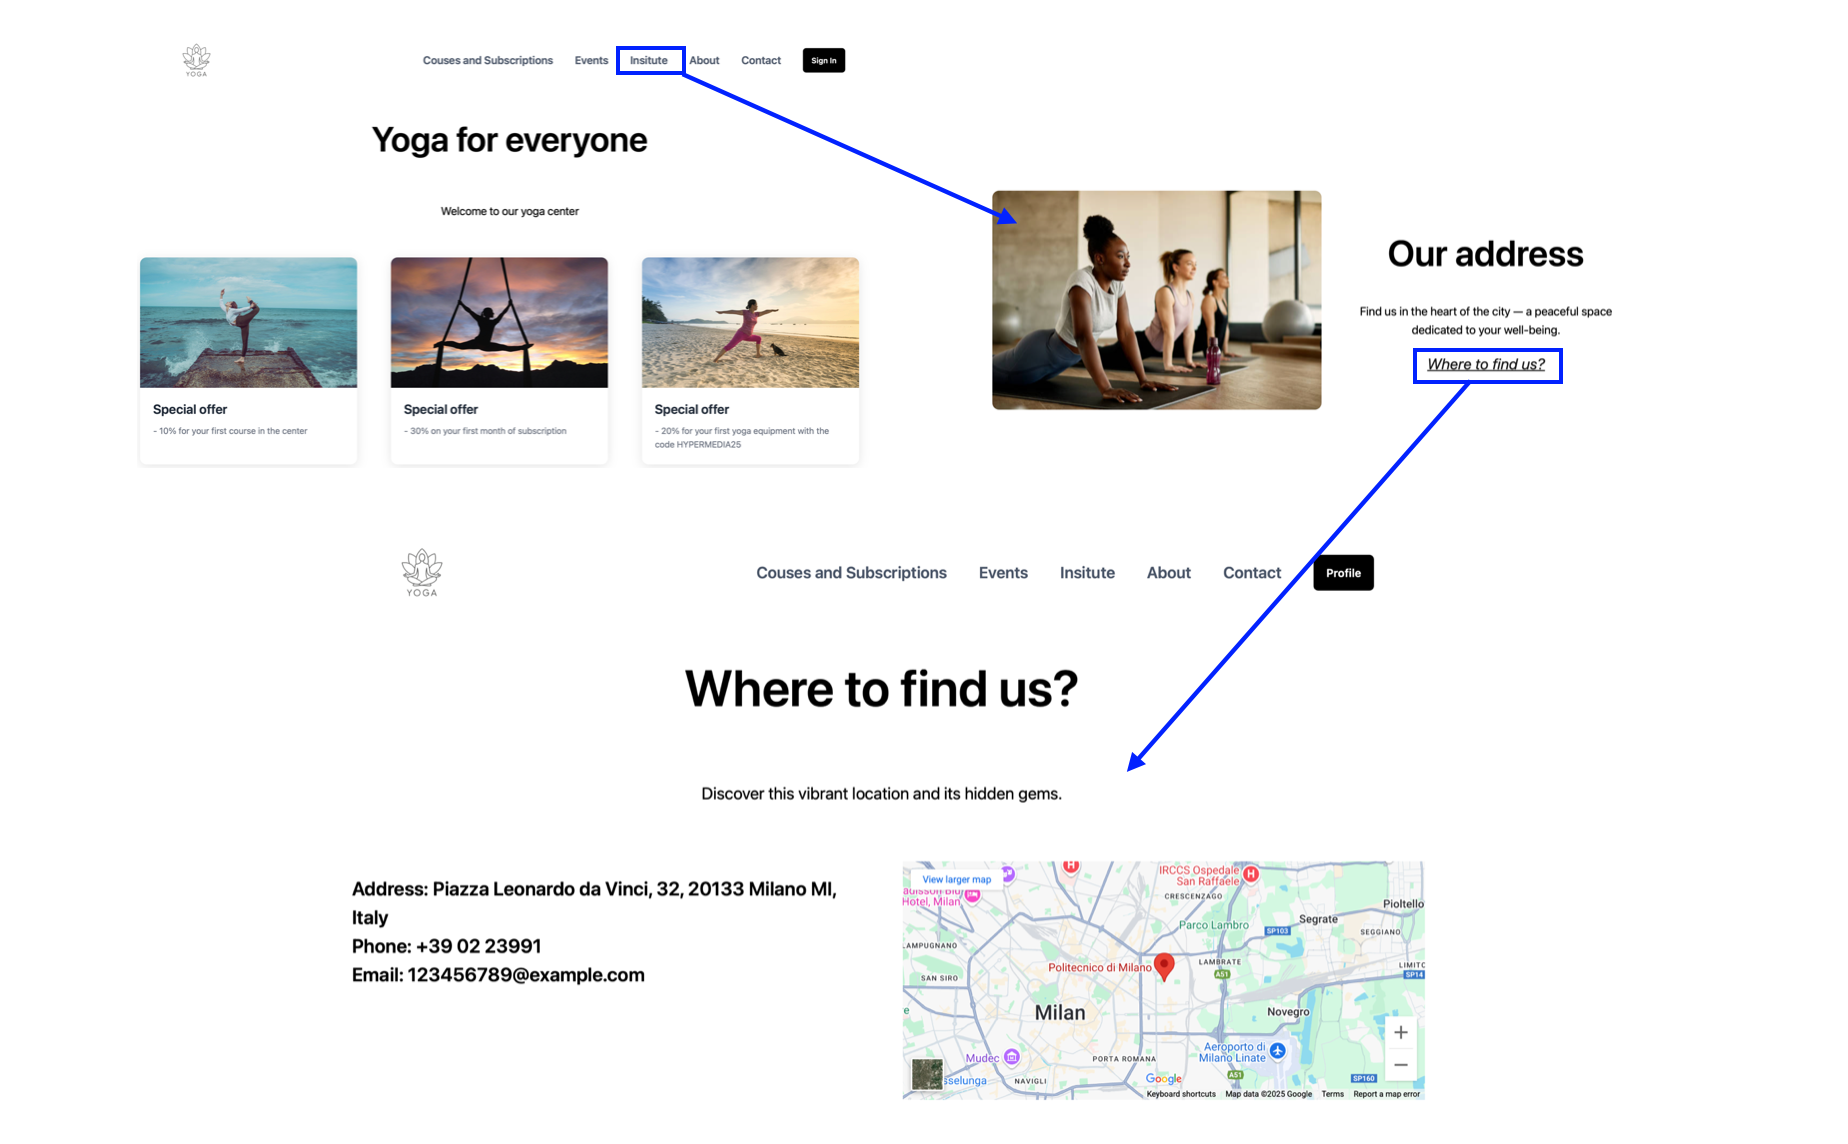
\includegraphics[width=0.9\textwidth]{asset/interactive_flow/location}
    \caption{Use case 1: Find the location of the center}
\end{figure}


\subsection{Use case 2}
\subsubsection{Textual narrative}

\usecasetable
    {Find somewhere to contact the center}
    {A potential customer seeking to reach the yoga center}
    {Their goal is to find a way to contact the center}
    {They access the web application from any personal device}
    {\begin{itemize}
         \item They access the \textit{Home page} of the website
         \item They navigate to the \textit{Contact} page using the navigation bar.
         \item They have the capability to compose messages via the contact form.
    \end{itemize}
    }


\subsubsection{Interaction Flow}
\begin{figure}[H]
    \centering
    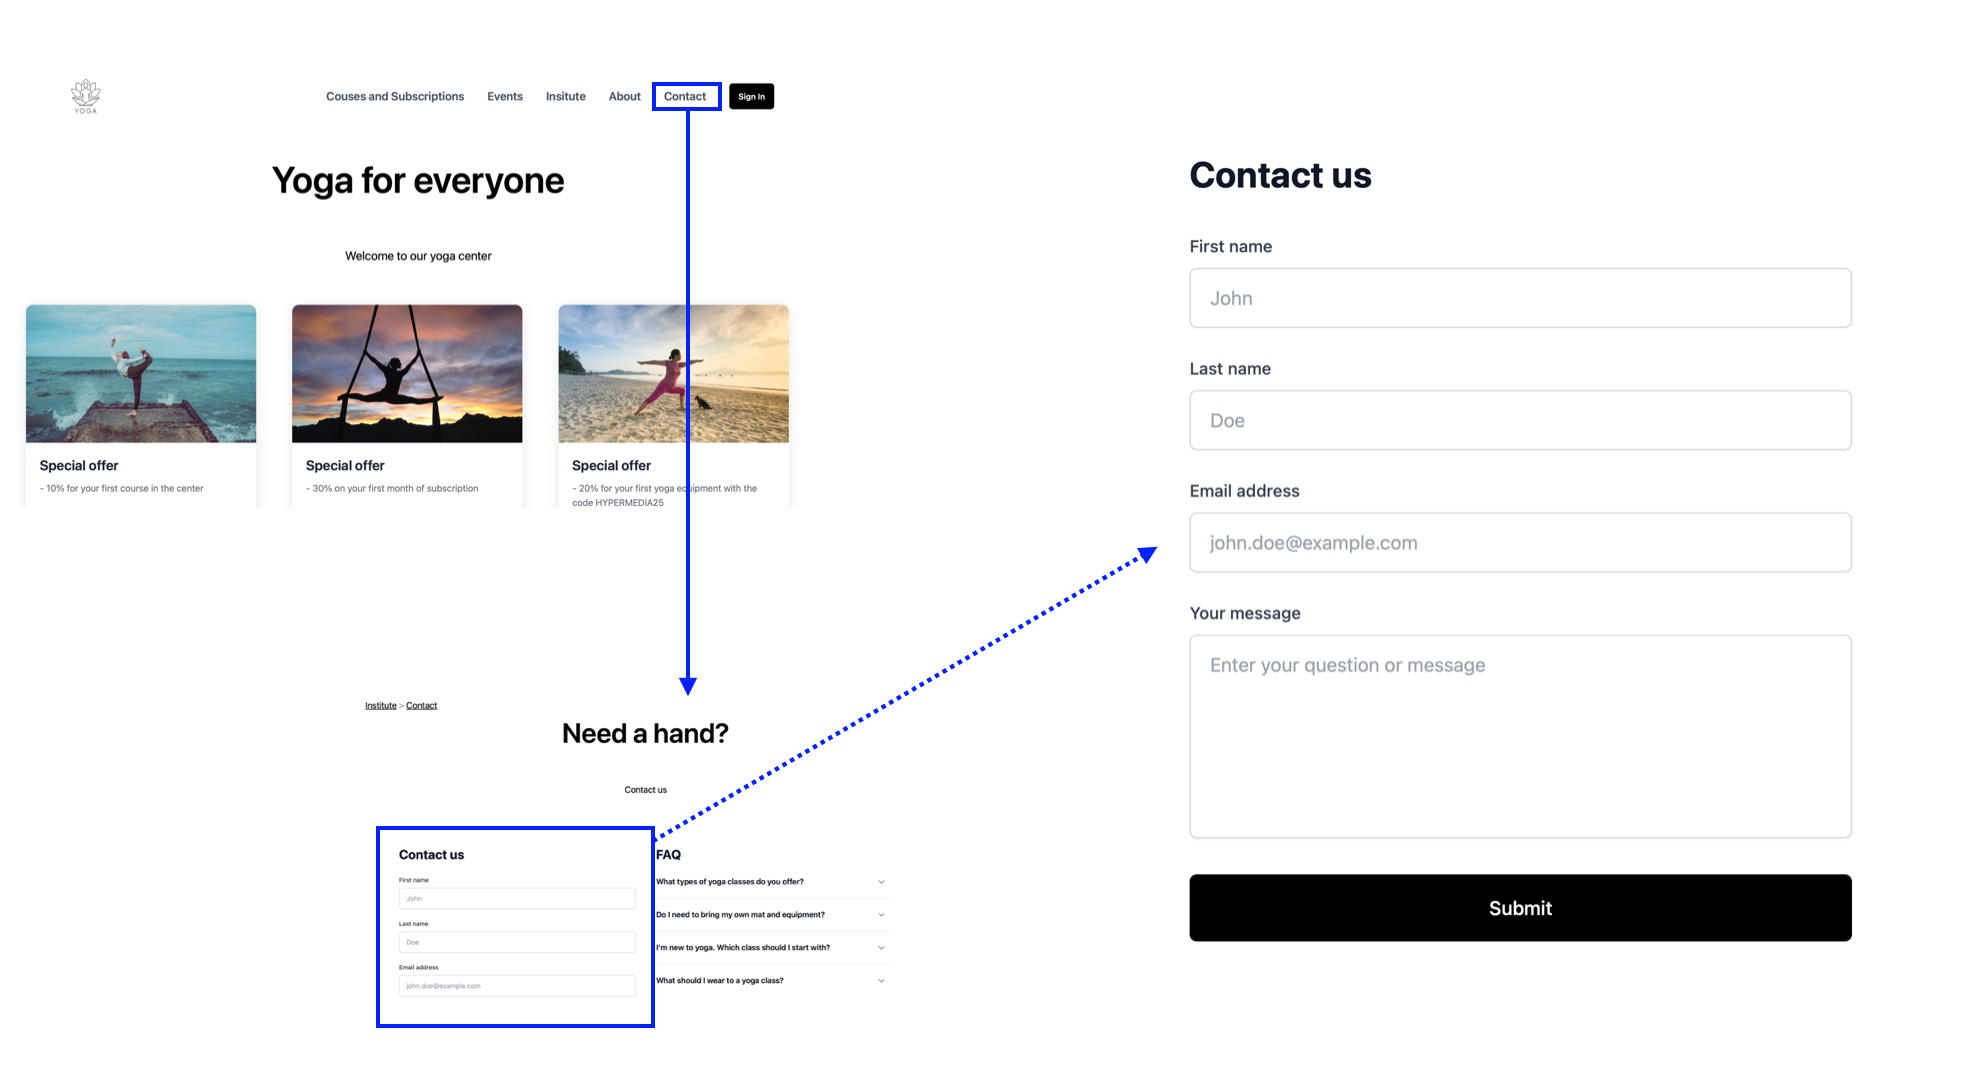
\includegraphics[width=0.9\textwidth]{asset/interactive_flow/contact}
    \caption{Use case 2: Find a way to contact the center}
\end{figure}


\subsection{Use case 3}
\subsubsection{Textual narrative}
\usecasetable
    {You want to know some exercices you can do at home}
    {A user seeking to practice at home}
    {Their goal is to find exercices and instructions to practice yoga at home}
    {They access the web application from any personal device}
    {\begin{itemize}
         \item They access the \textit{Home page} of the website
         \item They navigate to the \textit{About} page using the navigation bar. Then, they click on the
         \textit{Start now} button, which leads them to the \textit{Practice at home} page, where they can find a list of exercices, tutorials videos and some guidelines. Alternatively, they can access the \textit{Practice at home} page directly via the navigation bar.
    \end{itemize}
    }

\subsubsection{Interaction Flow}
\begin{figure}[H]
    \centering
    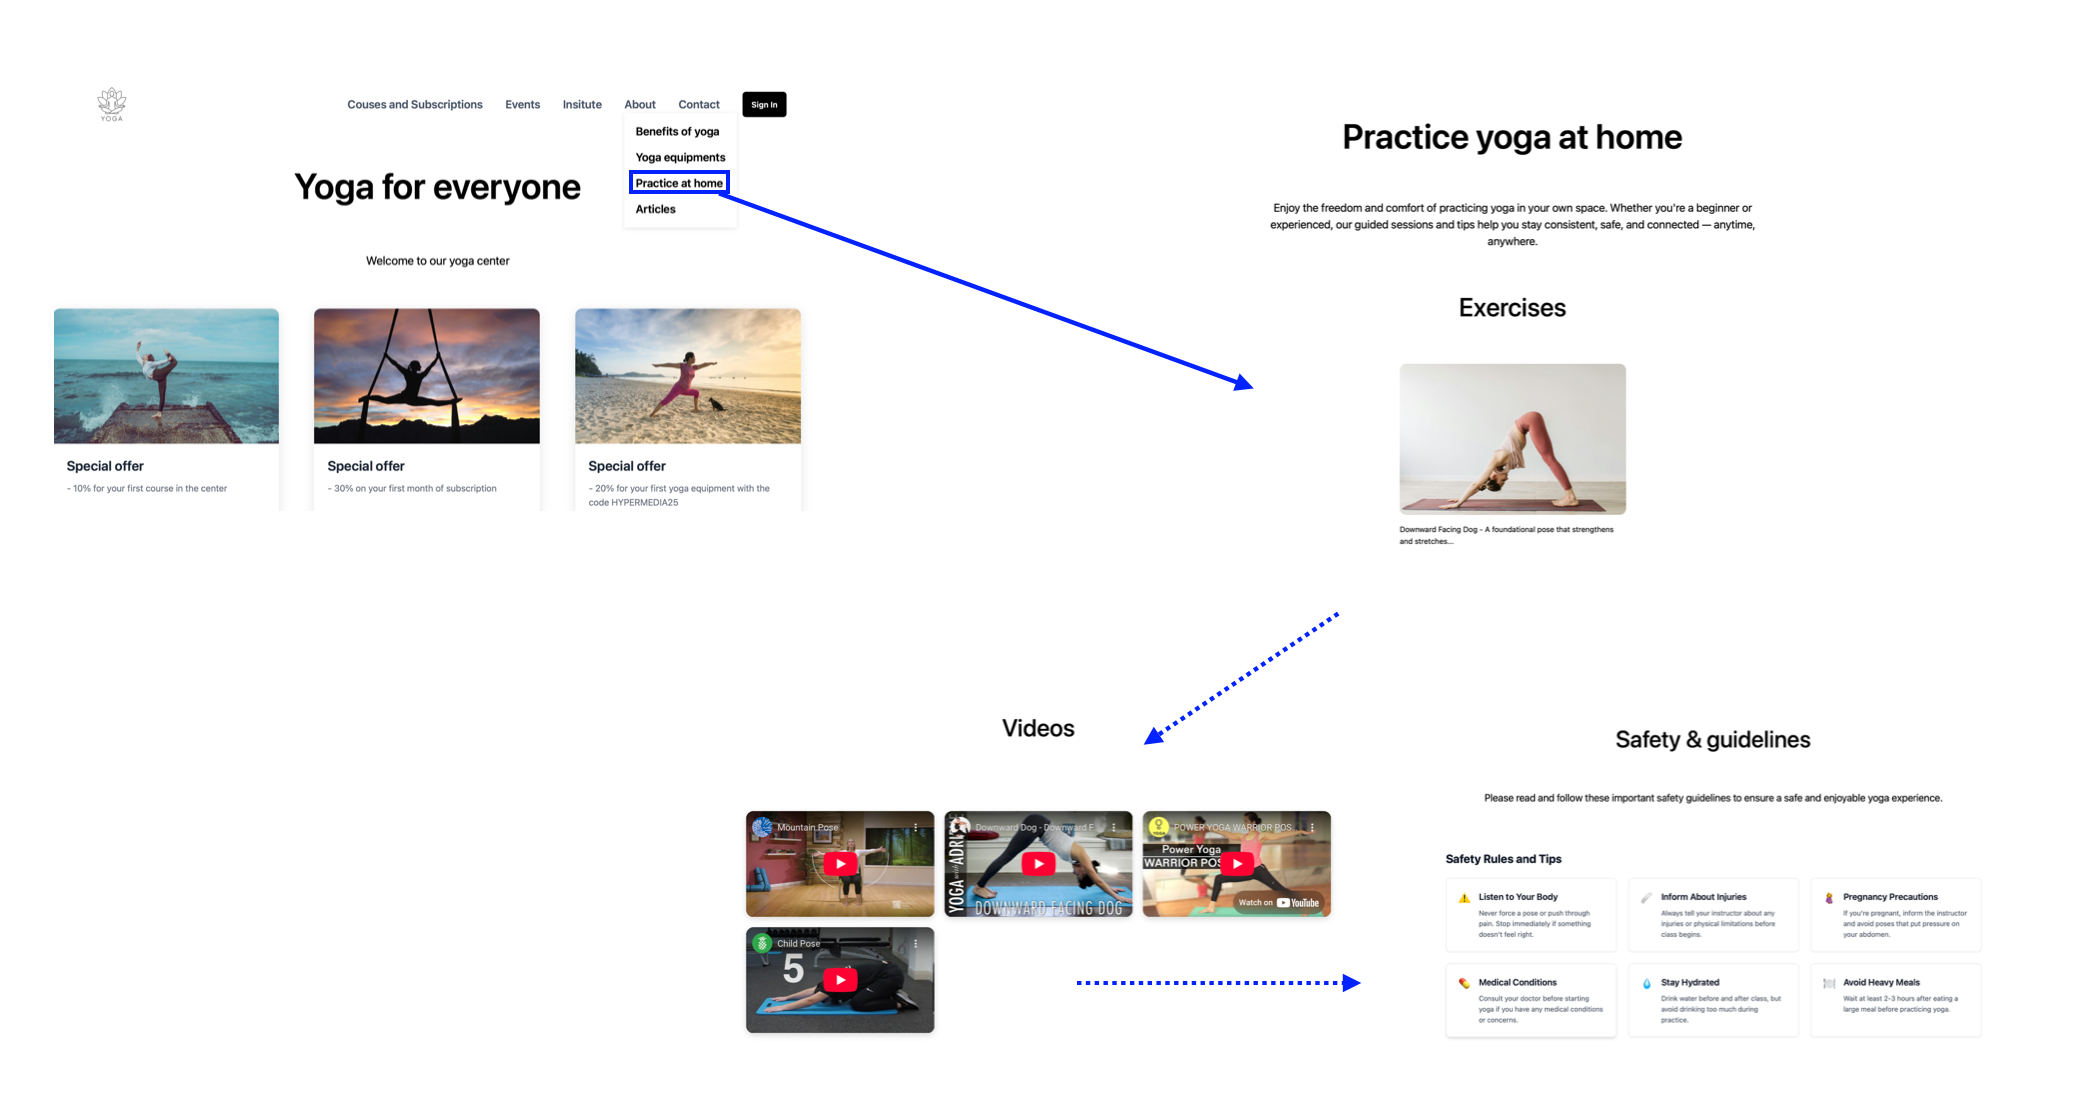
\includegraphics[width=0.9\textwidth]{asset/interactive_flow/practice}
    \caption{Use case 3: Find a way to practice yoga at home}
\end{figure}

\subsection{Use case 4}
\subsubsection{Textual narrative}
\usecasetable
    {Your friend recommanded you their favorite teacher, \textit{Chloe Dubois}, and you want to try some courses with her. Find her courses and then find the conditions to participate at 3 courses of her at the best price.}
    {A new visitor who heard about the yoga center through a friend. They are curious and motivated to try classes with a specific teacher and want to explore flexible options to attend three of her sessions at the best price.}
    {Their goal is to find the most affordable way to enroll in Chloe Dubois’s courses}
    {They access the web application from any personal devicer}
    {\begin{itemize}
         \item They access the \textit{Home page} of the website
         \item They navigate to the \textit{Institute} page using the navigation bar. Then, they click on the
                \textit{See your teachers} button, which leads them to the \textit{Teachers} page, where they can find all the
                center's teachers. Alternatively, they can access the \textit{Teachers} page directly via the navigation bar by clicking the \textit{The team} button.
         \item They click on \textit{Chloe Dubois' card} in order to see her profile and all her courses
         \item The can click on any \textit{course card} to see price and description
    \end{itemize}
    }

\subsubsection{Interaction Flow}




%You are looking for something to do on Tuesday afternoon, find which courses are given
%You are looking for an event on next Hollydays, find which event takes place between June 7th and June 12th
